\documentclass{article}
\usepackage{graphicx}
\usepackage{amsmath}
\usepackage{amsfonts}
\usepackage{bookmark}
\usepackage{booktabs}
\usepackage{exercises}
\graphicspath{ {./images/8.3} }
\usepackage{indentfirst}
\usepackage{amsthm}
\usepackage{yhmath}
\usepackage{geometry}
\usepackage{placeins}
\usepackage{csquotes}
\usepackage{pgfplots}
\newcommand*{\oldneg}{\mathord{\sim}}
\newcommand\showdiv[1]{\overline{\smash{)}#1}}
\newcommand\Mydiv[1]{%
\smash{\raise.3ex\hbox{$\big)$}}\mkern-8mu
        \overline{\enspace\strut#1}}
\setlength{\tabcolsep}{5pt}
\theoremstyle{definition}
\newtheorem{definition}{Definition}

\setlength{\parindent}{.5in}
\setlength{\parskip}{12pt}
\renewcommand{\arraystretch}{2}
\geometry{margin=1in}
\newcommand{\?}{\stackrel{?}{=}}
\pgfplotsset{width=7cm,compat=1.18}\usepgfplotslibrary{statistics}

\title{8.3 Answers}
\begin{document}
\maketitle

\section*{1}
The radius of a circle is the distance from any point on the circle to a fixed point called the circle's center.

\section*{2}
The slope of a line tangent to a circle and the slope of the radius at the point of tangency are perpendicular (that is, they are negative reciprocals).

\section*{3}
C

\section*{4}
E

\section*{5}
A

\section*{6}
D

\section*{7}
F

\section*{8}
B

\section*{19}
The equation is \[ 4x^2+4y^2=128 \] \[ 4(x^2+y^2)=128 \] \[ x^2+y^2=32 \] meaning the radius of the circle is 
$\sqrt{32}=4\sqrt{2}$:\newline
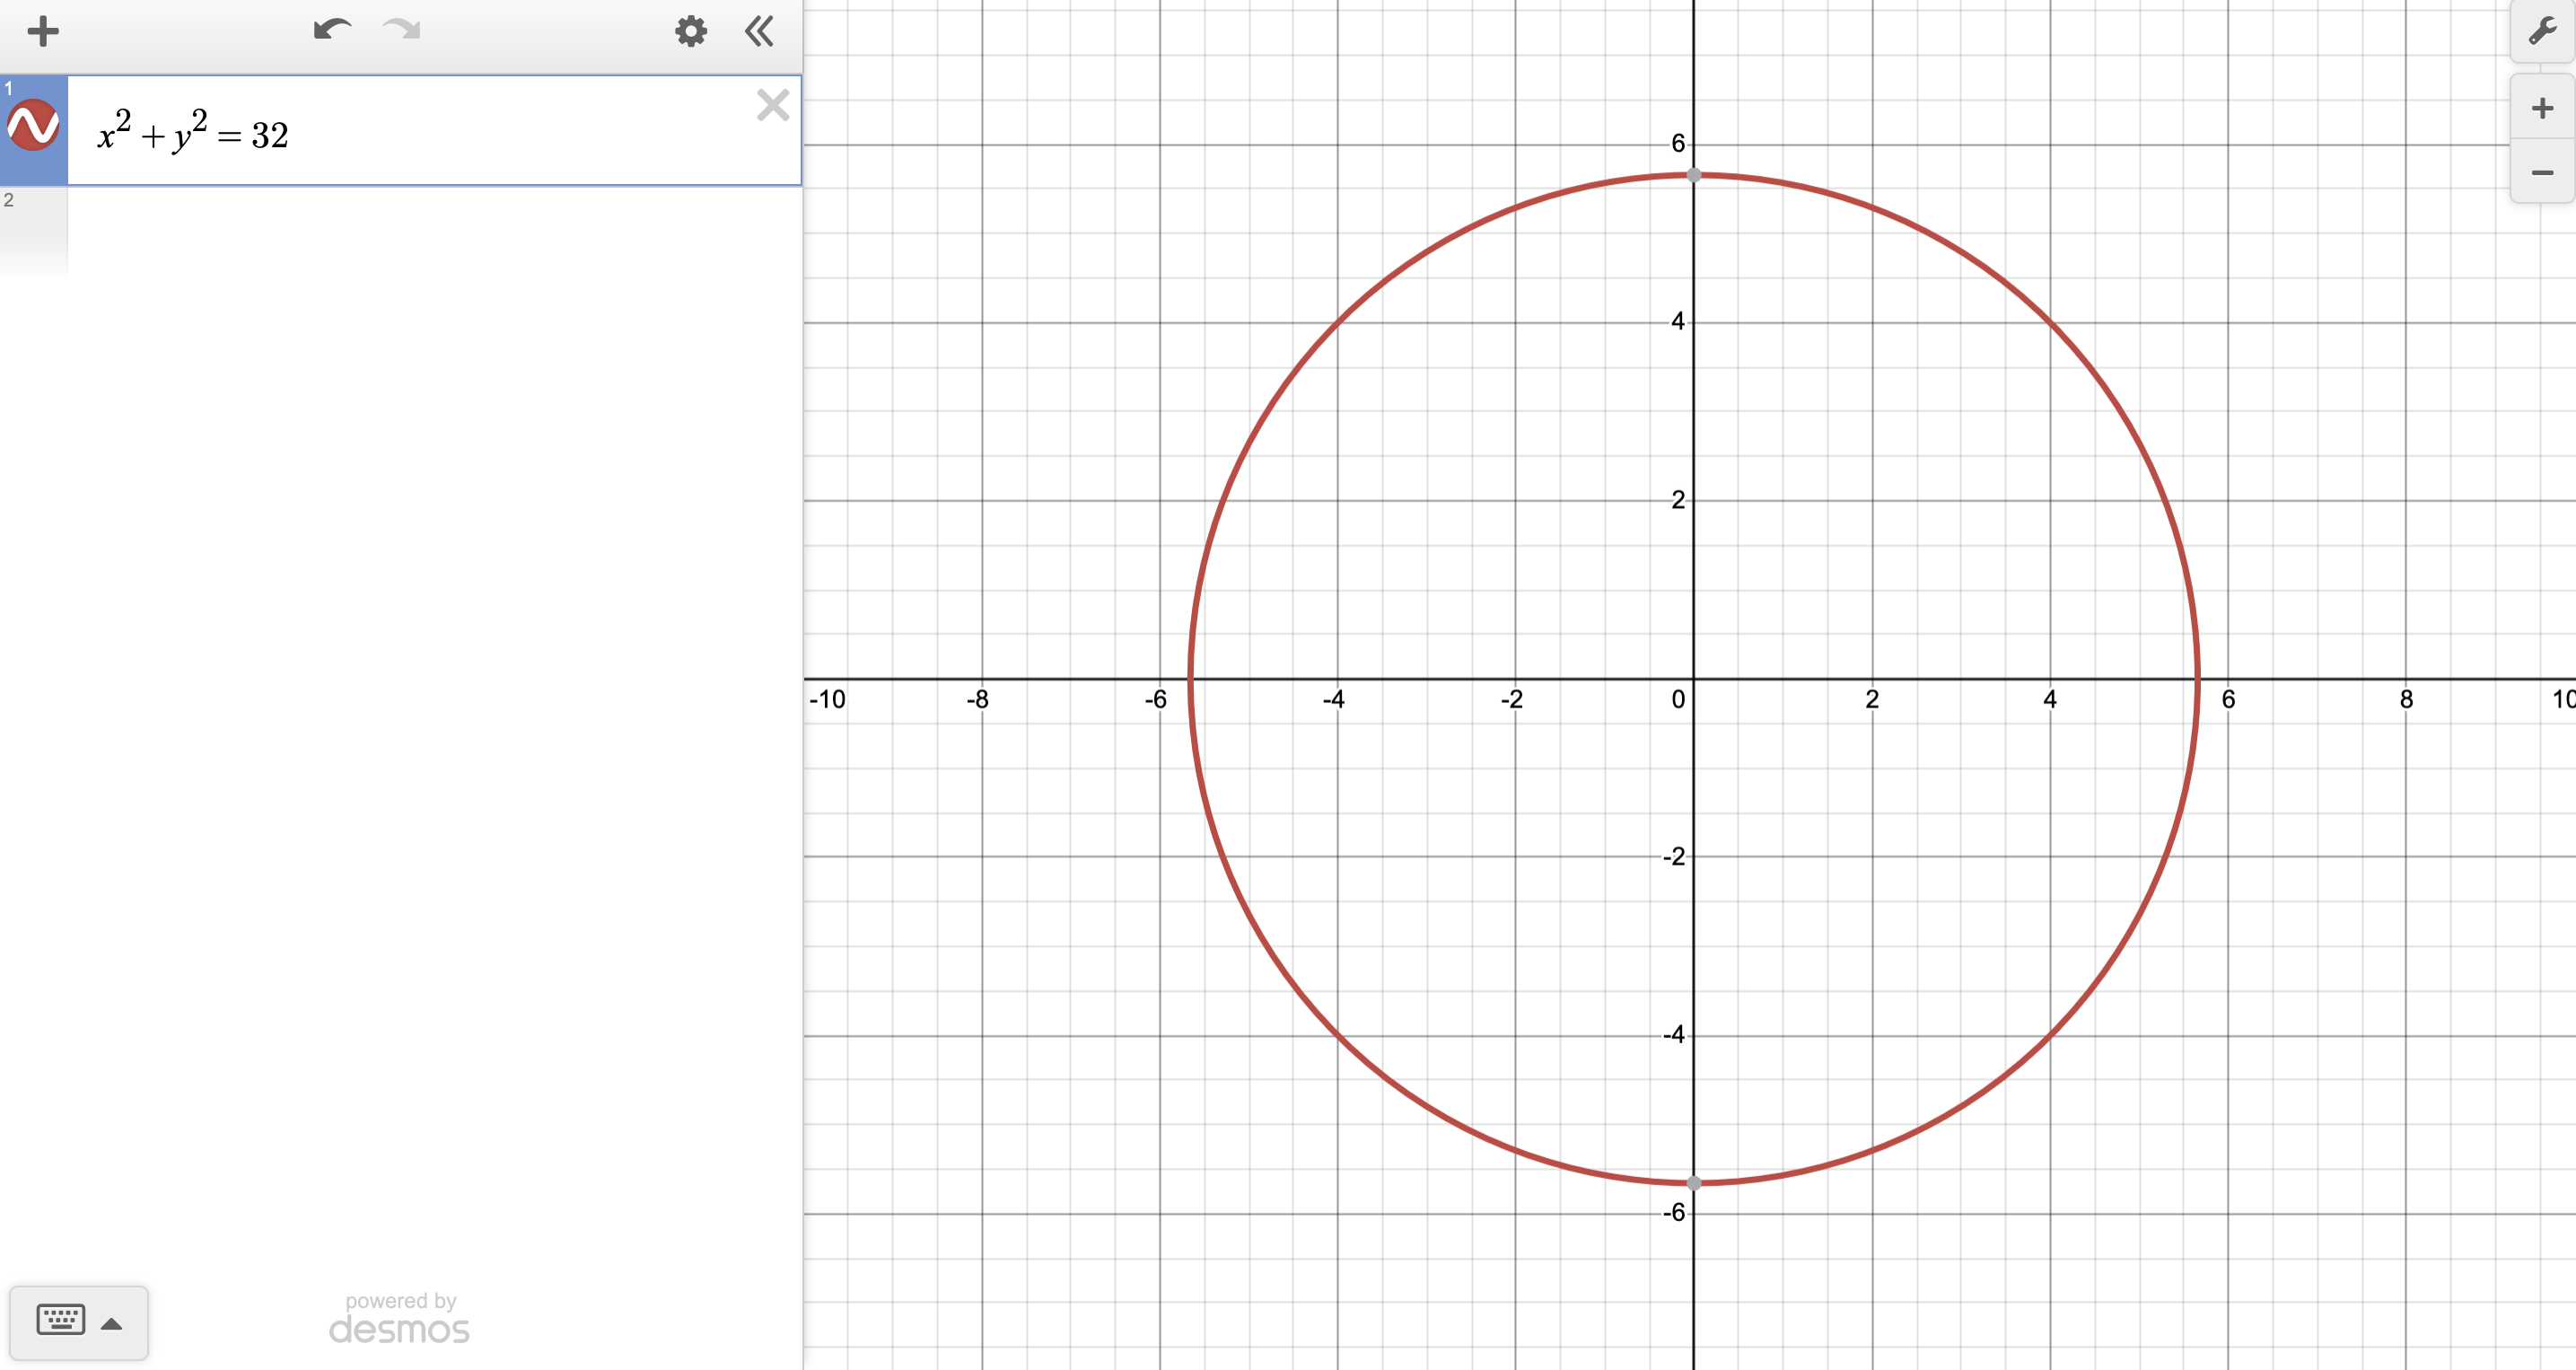
\includegraphics[width = 4in]{19}

\section*{20}
The equation is \[ 8x^2+8y^2=192 \] \[ x^2+y^2=24 \] meaning the radius of the circle is $\sqrt{24}=2\sqrt{6}$:\newline
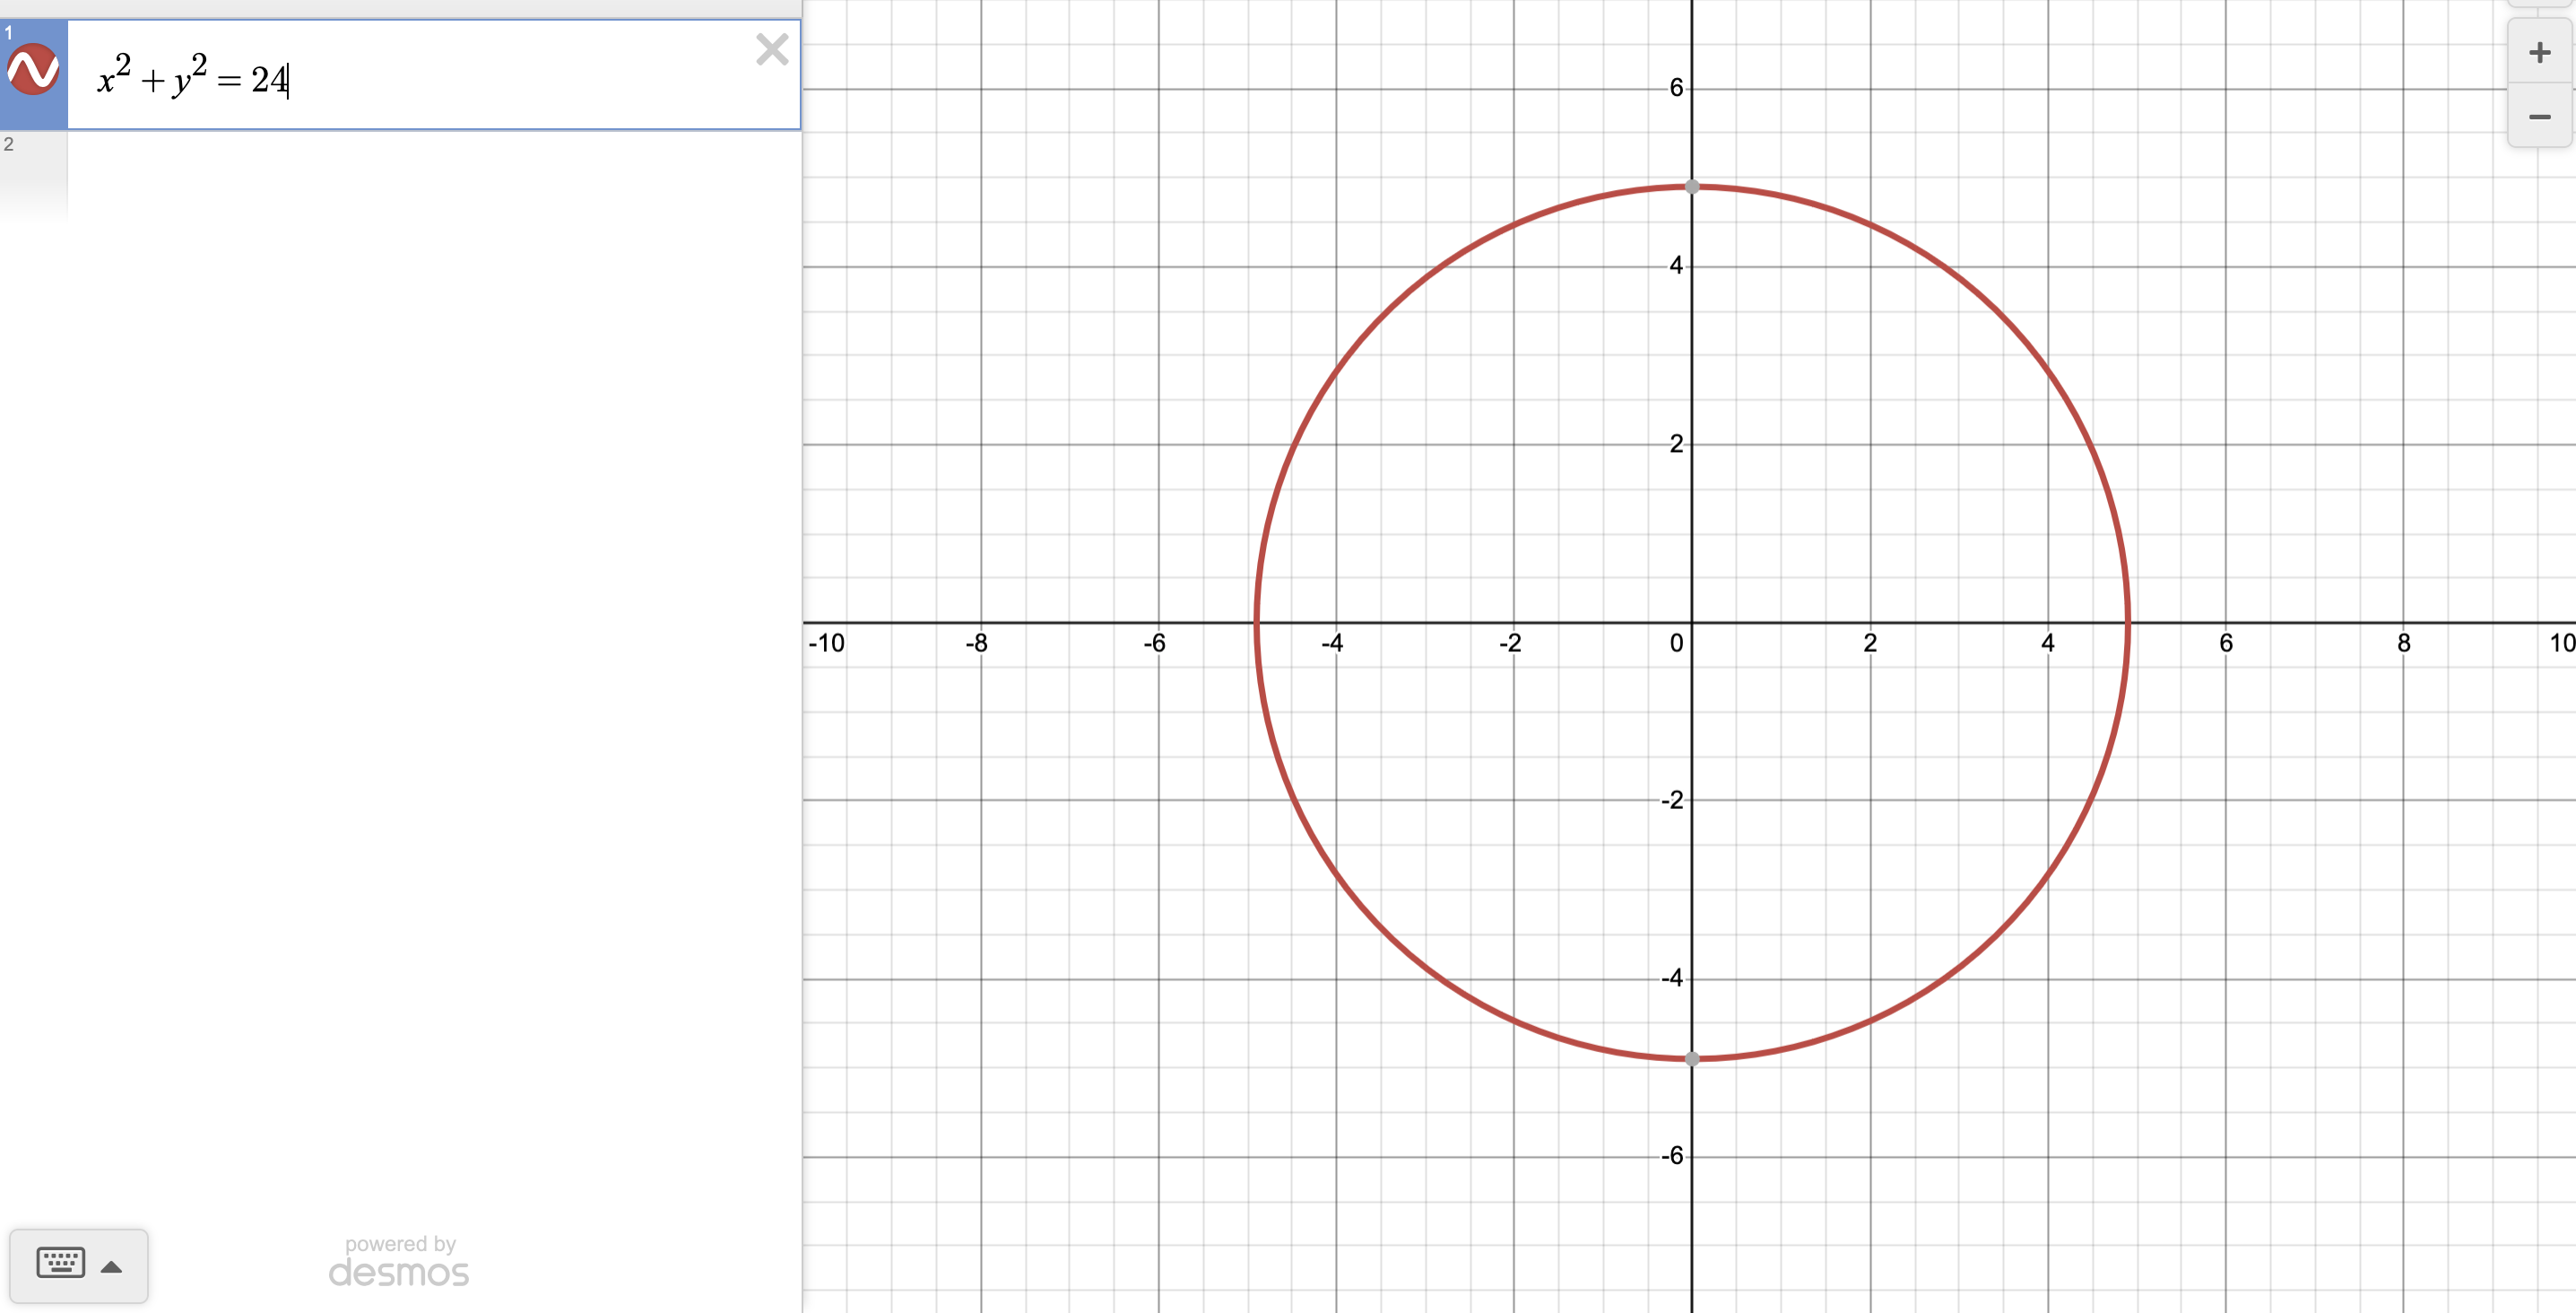
\includegraphics[width = 4in, height = 4in]{20}

\section*{21}
\[ 3x^2+3y^2=54 \] \[ 3(x^2+y^2)=54 \] \[ x^2+y^2=18 \] Thus $r=\sqrt{18}=3\sqrt{2}$. A

\section*{27}
$x^2+y^2=(\sqrt{15})^2=15$

\section*{28}
$x^2+y^2=(5\sqrt{2})^2=50$

\section*{29}
$x^2+y^2=(4\sqrt{6})^2=96$

\section*{30}
The equation for a circle centered at the origin is $x^2+y^2=r^2$ where $r$ is the radius. In the solution to this problem, the answer was given as 
$x^2+y^2=r$, not $r^2$, which is incorrect. Thus the answer should instead be $x^2+y^2=12^2=144$

\section*{40}
We know that \[ 5^2+(-12)^2=r^2 \] \[ 169=r^2 \] and thus the equation is $x^2+y^2=169$.

\section*{41}
We know that \[ (-11)^2+(-11)^2=r^2 \] \[ 242=r^2 \] and thus the equation is $x^2+y^2=242$.

\section*{42}
We know that \[ 9^2+40^2=r^2 \] \[ 1681=r^2 \] and thus the equation is $x^2+y^2=1681$.

\section*{43}
We know that \[ 4^2+(-6)^2=r^2 \] \[ 52=r^2 \] and thus the equation is $x^2+y^2=52$. C

\section*{51}
We know that the equation of the line tangent to the given circle at point $(-5,9)$ is perpendicular to the slope from the center to that point. 
The slope of that line is $\frac{9-0}{-5-0}=-\frac{9}{5}$. Thus the slope of the tangent line is $\frac{5}{9}$, meaning the equation for the line tangent to the circle 
at point $(-5,9)$ is:
\[ y-9=\frac{5}{9}(x+5) \]
\[ y=\frac{5}{9}x+\frac{106}{9} \]

\section*{52}
The slope of the line from the center of the circle to the point $(15,5)$ is $\frac{5-0}{15-0}=\frac{1}{3}$. Thus the slope of the line tangent to the circle at 
that point is $-3$, meaning the equation for that tangent line is:
\[ y-5=-3(x-15) \]
\[ y=-3x+50 \]

\section*{60}
To show that the angle inscribed in the semicircle is a right angle, we need to show that the lines forming it are perpendicular, that is, their slopes are negative reciprocals.
The slope of the frist line is $\frac{y-0}{x+r}=\frac{y}{x+r}$ while the slope of the second line is $\frac{0-y}{r-x}=-\frac{y}{r-x}$. Multiplying these two slopes together 
yields \[ \frac{y}{x+r}\times -\frac{y}{r-x}=-\frac{y^2}{r^2-x^2} \] We need to show that this is equal to $-1$ (that is, that they are negative reciprocals). Consider the 
distance from the center of the circle (at the origin) to $(x,y)$. It is $\sqrt{y^2+x^2}$. But this distance is just the radius $r$. Thus 
$r^2=y^2+x^2$. Hence:
\[ -\frac{y^2}{r^2-x^2}=-\frac{y^2}{y^2+x^2-x^2}=-\frac{y^2}{y^2}=-1 \] thus proving that the two lines are perpendicular.

\section*{61}
We are given two congruent circles passing through the others center. Thus they have the same radius $r$. Now, we can form two identical right triangles with the following 
sides: $r,\frac{r}{2},\frac{l}{2}$ where $r$ is the hypotenuse. Thus \[ (\frac{r}{2})^2+(\frac{l}{2})^2=r^2 \]
\[ \frac{r^2}{4}+\frac{l^2}{4}=r^2 \] \[ \frac{l^2}{4}=\frac{3r^2}{4} \] \[ l^2=3r^2 \] \[ l=r\sqrt{3} \]

\section*{64}
We are given that the appliance store gives delivery within a 100 mile radius, meaning an equation for the circle formed by this coverage is $x^2+y^2=100^2$ and 
thus an equation for which points are within range is $x^2+y^2<100^2=10000$. Thus D is the correct answer, as 
$75^2+70^2=10525>10000$, meaning it is not in range.

\section*{66}
We are given a circular tunnel with an 8 foot diameter. We are also given a 6-foot-wide walkway. We can let the circular tunnel have its center at the origin. Thus 
it can be modeled by the equation $x^2+y^2=4^2$. Now, the endpoints of this walkway have $x$-coordinates of $\pm 3$. Thus the $y$-coordinates of these endpoints are:
\[ 3^2+y^2=16 \] \[ y^2=7 \] \[ y=\pm\sqrt{7} \] The positive value does not make sense, as the walkway is at the bottom. Thus the endpoints are $(\pm 3,-\sqrt{7})$. 
We know that the radius of the tunnel is 4 feet. Thus, when one is standing on the walkway, they will be able to stand up $4+\sqrt{7}\approx 6.6$ feet. Hence a person who is 
6.2 feet tall will be able to stand on the walkway without ducking. 

\section*{67}
What it means for the circles to have the least amount of overlap is that the two circles intersect when $y=4.5$. We let the first circle be centered at the origin, meaning 
it has an equation of $x^2+y^2=6^2$. Then the second circle has an equation of $(x-h)^2+y^2=6^2$ where $h$ is the distance between the first and second circles. Thus 
\[ x^2+4.5^2=6^2 \] \[ x=\pm\sqrt{15.75} \] and \[ (x-h)^2+4.5^2=6^2 \] \[ x=h\pm\sqrt{15.75} \] Now, because $x=\pm\sqrt{15.75}$ corresponds to the first circle, 
$x=\sqrt{15.75}$. Also, because $x=h\pm\sqrt{15.75}$ corresponds to the second circle, $x=h-\sqrt{15.75}$. Thus 
\[ \sqrt{15.75}=h-\sqrt{15.75} \] \[ h=2\sqrt{15.75}\approx 7.94 \] feet. 

\section*{69}
We are given a circle with a radius of 40 miles and another circle with a radius of 60 miles. We are also given that the distance between them is 80 miles, and that 
the person is driving 10 miles above the centers of the two circles, and that they are driving at 60 miles per hour. We let the circle with a radius of 40 miles be centered 
at the origin, meaning the equation for the points in the circle is $x^2+y^2<40^2=1600$. Then the equation for the points in the second circle is $(x-80)^2+y^2<60^2=3600$. 
Thus we need to determine what values of $x$ are in both of the circles when $y=10$: 
\[ x^2+100<1600 \] \[ x^2<1500 \] \[ -\sqrt{1500}<x<\sqrt{1500} \] \[ -38.73<x<38.73 \] and \[ (x-80)^2+100<3600 \] \[ -\sqrt{3500}<x-80<\sqrt{3500} \]
\[ 20.84<x<139.16 \] Thus the driver is in range of both towers when $20.84<x<38.73$. The distance while in range of both towers is therefore $38.73-20.84=17.89$ miles, 
meaing the time spent driving within range of both towers is $\frac{17.89}{60}\approx 0.30$ hours or about $18$ minutes.

\end{document}
